\documentclass[aspectratio=169,t,11pt,table]{beamer}
\usepackage{../../slides}
\usepackage{../../math}

% Optionally define `accent`/`accent2` colors for theme customization
% I recommend changing the top slider on this: https://hslpicker.com/#1e9400
\definecolor{accent}{HTML}{9D2235}
\definecolor{accent2}{HTML}{2B5269}

\title{Topic 1: Introduction to Forecasting}
\subtitle{\it  ECON 4753 — University of Arkansas}
\date{Fall 2024}
\author{Prof. Kyle Butts}

\begin{document}

% ------------------------------------------------------------------------------
\begin{frame}[noframenumbering,plain]
\maketitle

% \bottomleft{\footnotesize $^*$A bit of extra info here. Add an asterich to title or author}
\end{frame}
% ------------------------------------------------------------------------------


% ------------------------------------------------------------------------------
\section{Forecasting}
% ------------------------------------------------------------------------------

\begin{frame}{Problem of Prediction}
  The goal of forecasting is to learn the relationship between \alert{input variables} and \alert{outcome variable(s)} so that we can \alert{predict} the outcome variables when we do not observe it. 
  \pause E.g.
  \begin{itemize}
    \item Learn about who are potential customers to advertise to based on their observable characteristics
    \begin{itemize}
      \item Input: observable characteristics
      \item Outcome: whether they purchase a product
    \end{itemize}
    
    \pause
    \item Predict values of a variable in the future, e.g. \alert{time-series} of stock prices
    \begin{itemize}
      \item Input: the time-period
      \item Output: stock price
    \end{itemize}
  \end{itemize}  
\end{frame}

\begin{frame}{Prediction model}
  We have an outcome variable $Y$ and a set of $p$ different predictor variables $X = (X_1, X_2, \dots, X_p)$. 
  \begin{itemize}
    \item For some observations we observe both $X$ and $Y$; this is essential to \alert{fit} the model
  \end{itemize}

  \bigskip
  We can write the model in a general form as
  $$
    Y = f(X) + \varepsilon,
  $$
  where $f$ is some unknown function of $X$ and $\varepsilon$ is the \alert{error term} which we assume is unrelated to $X$ and mean zero.
\end{frame}

\imageframe{figures/f_examples_plot_raw.pdf}
\imageframe{figures/f_examples_plot_pred_1.pdf}
\imageframe{figures/f_examples_plot_pred_2.pdf}
\imageframe{figures/f_examples_plot_pred_3.pdf}
\imageframe{figures/f_examples_plot_pred_4.pdf}

\begin{frame}{Advertising Example}
  Let's given an example. Say you're a business and you want to use advertising to boost sales. You have a bunch of different markets (e.g. cities) and you have data on how you've spent your advertising budget in those markets and the sales in that market
\end{frame}

\begin{frame}{Advertising Example}{Single-variable predictors}
  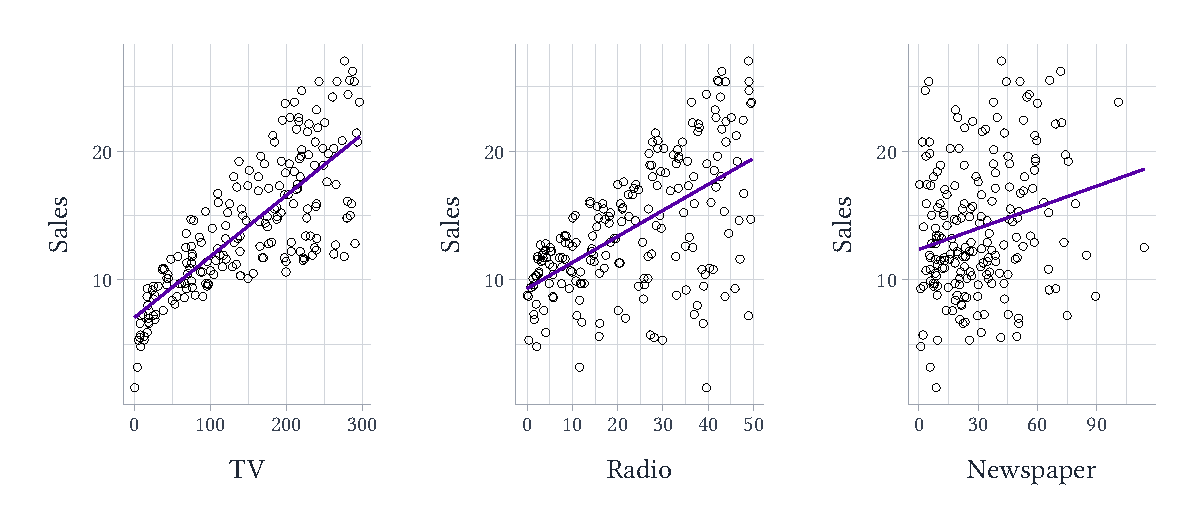
\includegraphics[width=\textwidth]{figures/sales_bivariate.pdf}
\end{frame}

\begin{frame}{Advertising Example}
  We see that sales are higher in markets that have spending on TV, Radio, and Newspaper ads separately. 
  
  \pause
  \bigskip 
  These single scatter plots with line of best-fits are a somewhat poor model:
  \begin{itemize}
    \item Are there synergies between different advertising strategies (are they substitutes or complements to one another)?
    \item Do places with more TV ads also have more radio ads? Then how can we tell if it is TV ads that are helping or if it is really radio ads 
  \end{itemize}

  \pause\bigskip
  \alert{Key takeaway:} Forecasting models get better the more carefully you think about the context you are in
\end{frame}

\begin{frame}{Error term}
  \begin{center}
    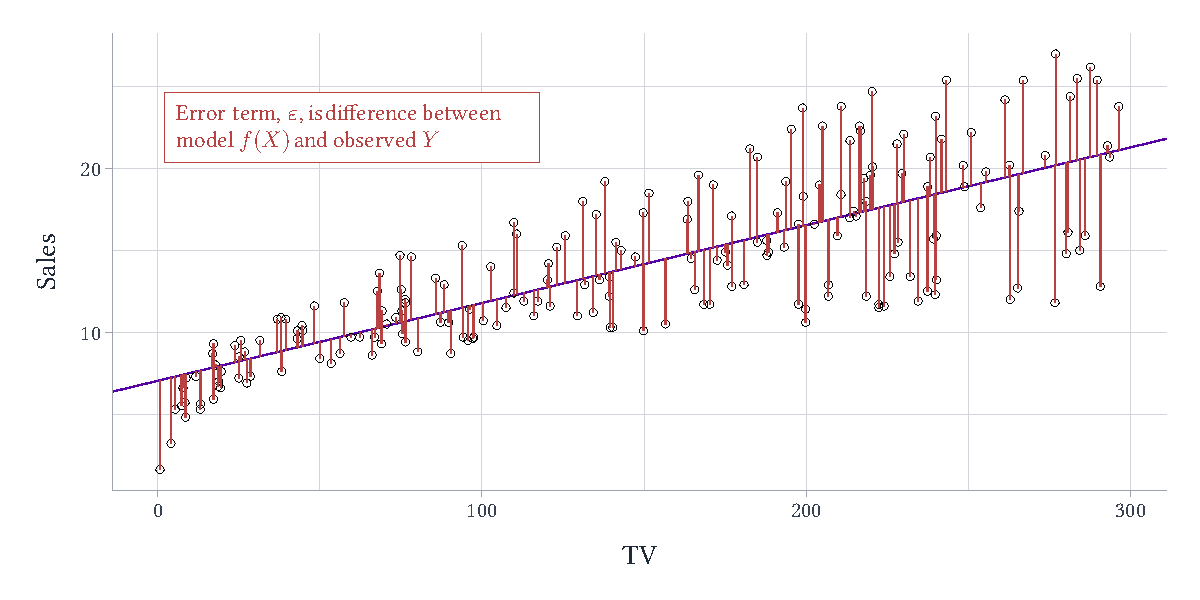
\includegraphics[width=0.9\textwidth]{figures/sales_tv_error_term.pdf}
  \end{center}
\end{frame}

\begin{frame}{Error term}
  In the previous figure, we were able to determine $\varepsilon$ because we assumed we \emph{knew} the model $f$ and therefore could observe $f(X)$ for each market.

  \bigskip
  In reality, we do not know $f$ and can never observe $\varepsilon$. But, we can try and estimate it ...
\end{frame}

% ------------------------------------------------------------------------------
\section{Goals of Forecasting}
% ------------------------------------------------------------------------------

\begin{frame}{Why estimate $f$?}
  There are two related reasons to try and predict $f$:
  \begin{enumerate}
    \item Predict $y$ as good as possible (\alert{prediction})
    \begin{itemize}
      \item Think of prediction as a `black box' where the goal is to do as good of a job at predicting $y$ as possible
    \end{itemize}
    
    \item Understand the relationship between $x$ and $y$ (\alert{inference})
    \begin{itemize}
      \item If our goal is being able to describe the relationship between $x$ and $y$.
    \end{itemize}
  \end{enumerate}
\end{frame}

\begin{frame}{Model Flexibility}
  There is a limit to how \alert{flexible} we can make our model
 
  \bigskip
  \begin{enumerate}
    \item If our goal is prediciton, we only have a finite amount of data to use to fit the model, so there's a limit on how much we can learn
    \begin{itemize}
      \item Face the risk of \alert{overfitting} the data (chasing after the random noise $\varepsilon$)
    \end{itemize}
   
   \item If our goal is inference, then added flexibility is harder to summarize to stakeholders.
  \end{enumerate}
\end{frame}

\imageframe{figures/f_examples_plot_pred_4.pdf}


\section{Evaluating Models}

\begin{frame}{Prediction Error}
  Given our model, we will want to be able to evaluate how good our model does at predicting observations $y$

  \bigskip
  Define the \alert{prediction error} as 
  $$
    \hat{\varepsilon} = \underbrace{y}_{\text{true value}} - \underbrace{\hat{y}}_{\text{predicted value}}
  $$

\end{frame}

\begin{frame}{Prediction Error}
  $$
    \hat{\varepsilon} = \underbrace{y}_{\text{true value}} - \underbrace{\hat{y}}_{\text{predicted value}}
  $$

  \bigskip
  Large $\hat{\varepsilon}$ means you did a poor job of predicting that observation. That could be because
  \begin{enumerate}
    \item The linear model is bad at predicting $y$
    \item Or, the true noise $\varepsilon$ is making $y$ far away from the systematic component $f(X)$ for this observation
  \end{enumerate}
\end{frame}

\begin{frame}{Mean-square prediction error}
  To provide a summary measure of fit, we want to \emph{average} prediction error over many observations. This will find a `average' prediction error
  \begin{itemize}
    \item If we took the simple mean of prediction error, positive and negative prediction errors would cancel out
  \end{itemize}

  \pause
  \bigskip
  The \alert{mean-square (prediction) error} (MSE) is calculated as:
  \begin{equation}\label{eq:mspe}
    \text{MSE} \equiv \frac{1}{n} \sum_{i=1}^n \left( y_i - \hat{y}_i \right)^2 = \frac{1}{n} \sum_{i=1}^n \hat{\varepsilon}_i^2
  \end{equation}
  \begin{itemize}
    \item Average of squared prediction error
  \end{itemize}
\end{frame}

\begin{frame}{Mean-square prediction error}
  \begin{columns}[T]
    \begin{column}{.3\textwidth}\vspace*{-\bigskipamount}
      \begin{table}
\centering
\begin{tblr}[         %% tabularray outer open
]                     %% tabularray outer close
{                     %% tabularray inner open
colspec={Q[]Q[]Q[]},
row{even}={bg=black!5!white},
colsep = {1em},
}                     %% tabularray inner close
\toprule
$y_i$ & $\hat{y}_i$ & $\hat{\varepsilon}_i$ \\ \midrule %% TinyTableHeader
3.7 & 4.20 & \only<2>{0.5} \\
4.1 & 4.18 & \only<2>{0.08} \\
5.6 & 5.48 & \only<2>{-0.12} \\
2.9 & 3.29 & \only<2>{0.39} \\
8.8 & 8.81 & \only<2>{0.01} \\
\bottomrule
\end{tblr}
\end{table}

    \end{column}
    \hfill
    \begin{column}{.6\textwidth}
      Calculate mean-square prediction error:

      \only<2>{\begin{align*}
  \text{MSPE} &= \frac{1}{5} \left( 0.5^2 + 0.08^2 + -0.12^2 + 0.39^2 + 0.01^2 \right) \\
  &= 0.0846
\end{align*}}
    \end{column}
  \end{columns}
\end{frame}

\begin{frame}{In-sample vs. Out-of-sample prediction error}
  As a forecaster, you will \alert{fit} a model using a set of observations $\left\{ (x_1, y_1), \dots, (x_n, y_n) \right\}$. This is called the \alert{training data}.

  \bigskip
  We can calculate the \alert{in-sample MSE} by formula (\ref{eq:mspe}) averaging over all observations in the training data.
  \begin{itemize}
    \item This tells us how good we do at predicting the data \emph{we trained the model on}.
  \end{itemize} 
\end{frame}  

\begin{frame}{In-sample vs. Out-of-sample prediction error}
  If our goal is prediction, we really want to know how the model would predict on \emph{new} observations that we \emph{have not seen before}
  \begin{itemize}
    \item It is common to hold out a set of \alert{test data} that is NOT used for training the model, but just for evaluating it's performance
  \end{itemize}
\end{frame}

\begin{frame}{Why use `test data'?}
  It is common to try and `pick' from a set of models based on how they do at in-sample prediction:
  \begin{itemize}
    \item That is, select the model with the smallest \emph{in-sample MSE}. 
  \end{itemize}

  \pause
  \bigskip
  This is \emph{a bad thing to do}; by focusing on fitting the current sample very well, you are risking \alert{overfitting} the data
\end{frame}

\begin{frame}{Flexibility vs. Overfitting}
  \vspace{-\bigskipamount}
  \begin{center}
    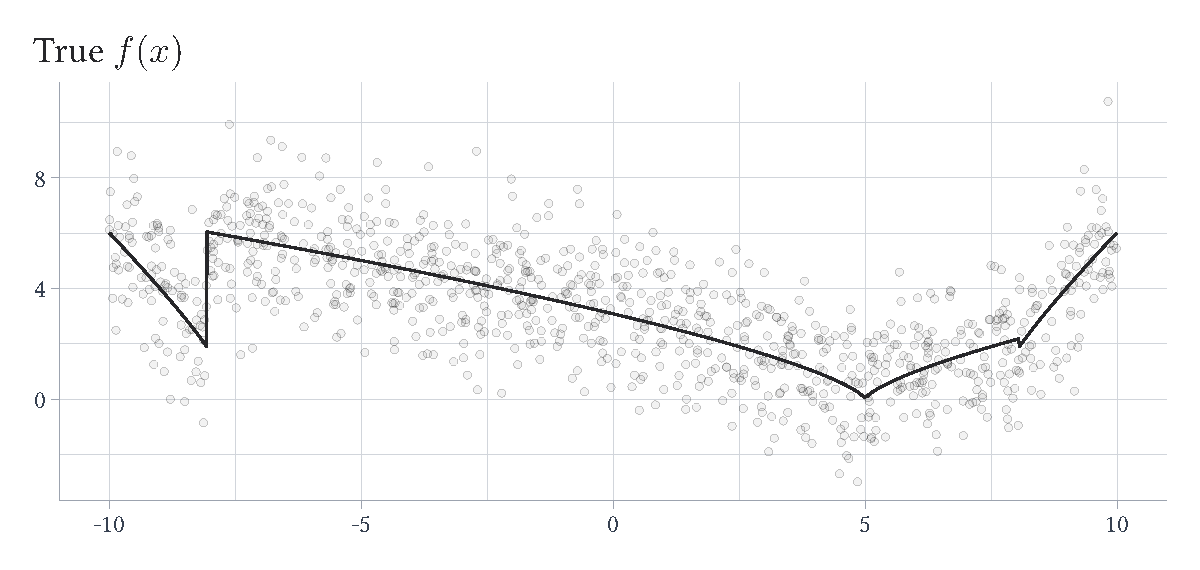
\includegraphics[width = \textwidth]{figures/f_examples_plot_dgp.pdf}
  \end{center}
\end{frame}

\begin{frame}{Flexibility vs. Overfitting}
  \vspace{-\bigskipamount}
  \begin{center}
    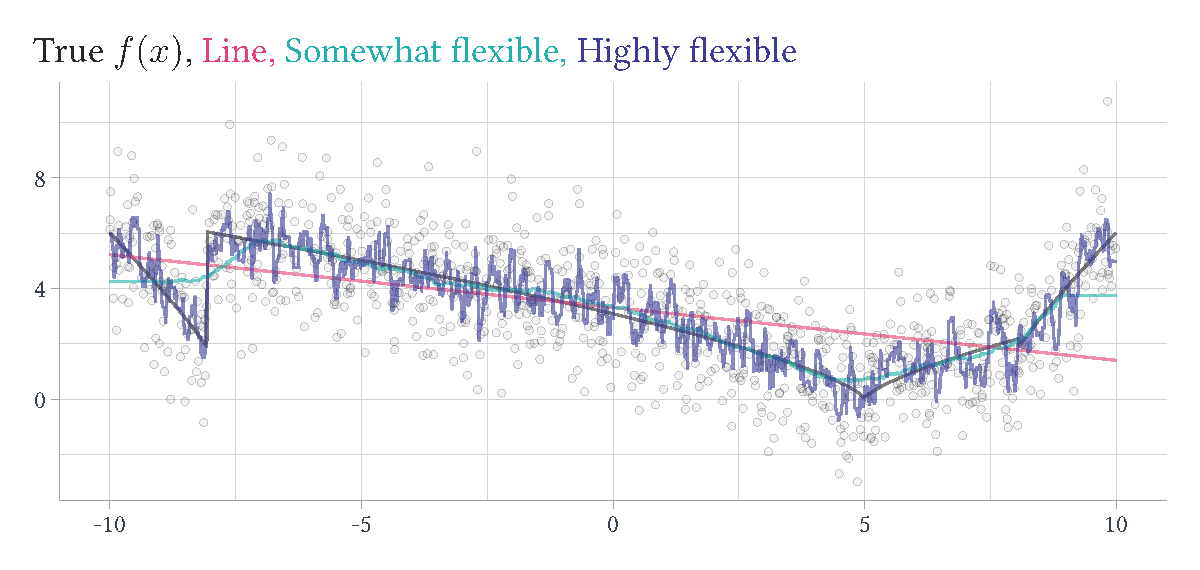
\includegraphics[width = \textwidth]{figures/f_examples_overfitting.pdf}
  \end{center}
\end{frame}

\begin{frame}{Flexibility vs. Overfitting}
  By making the model more and more \emph{flexible}, you risk overfitting more and more

  \begin{itemize}
    \item A solution is to evaluate your model fit using outside `testing data'
  \end{itemize}

  \pause
  \bigskip
  This technique is not as common when you care more about the associations between variables (interpreting the model)
  \begin{itemize}
    \item Not really a good reason other than "that is more complicated"
  \end{itemize}
\end{frame}


\begin{frame}{Bias-variance trade-off}
  This discussing of increasing flexiblity leading to increasing the noise of the model fit is a well-known problem. It is called the \alert{Bias-Variance Tradeoff}:
  \begin{enumerate}
    \item \alert{Bias}: When the model we fit, $\hat{f}(x)$, does a poor job fitting the true model $f(x)$
    
    \item \alert{Variance}: When the model we fit, $\hat{f}(x)$, is very variable across samples
    \begin{itemize}
      \item In repeated sampling, the model we estimate varies from estimate to estimate
    \end{itemize}
  \end{enumerate}

  \pause
  \bigskip
  This is a `trade-off'. To lower bias by adding flexibility, you're adding variance (noisiness) to the estimate 
\end{frame}





\section{Types of Data}

\begin{frame}{Cross-sectional Data}
  
  \begin{columns}[T]
    \begin{column}{.4\textwidth}
      \alert{Cross-sectional data} consists of many different \emph{units} viewed at a point in time:
    \end{column}
    \begin{column}{.6\textwidth}
      \vspace*{-\bigskipamount}
      \begin{table}
\centering
\begin{tblr}[         %% tabularray outer open
]                     %% tabularray outer close
{                     %% tabularray inner open
colspec={Q[]Q[]Q[]Q[]},
row{even}={bg=black!5!white},
colsep = {1em},
}                     %% tabularray inner close
\toprule
school\_id & avg\_sat\_math & pct\_white & pct\_black \\ \midrule %% TinyTableHeader
01M539 & 657 & 28.6\% & 13.3\% \\
02M294 & 395 & 11.7\% & 38.5\% \\
02M308 & 418 & 3.1\% & 28.2\% \\
02M545 & 613 & 1.7\% & 3.1\% \\
01M292 & 410 & 3.9\% & 24.4\% \\
01M696 & 634 & 45.3\% & 17.2\% \\
\bottomrule
\end{tblr}
\end{table}

    \end{column}
  \end{columns}
\end{frame}

\begin{frame}{Time-series Data}
  \begin{columns}[T]
    \begin{column}{.4\textwidth}
      \alert{Time-series data} consists of a single observational unit viewed over multiple points in time:
    \end{column}
    \begin{column}{.6\textwidth}
      \vspace*{-\bigskipamount}
      \begin{table}
\centering
\begin{tblr}[         %% tabularray outer open
]                     %% tabularray outer close
{                     %% tabularray inner open
colspec={Q[]Q[]Q[]Q[]Q[]},
row{even}={bg=black!5!white},
colsep = {1em},
}                     %% tabularray inner close
\toprule
month & day & hour & bikers & temp \\ \midrule %% TinyTableHeader
1 &  1 & 0  & 16 & 0.24 \\
1 &  1 & 1  & 40 & 0.22 \\
1 &  1 & 2  & 32 & 0.22 \\
$\vdots$ & $\vdots$ & $\vdots$ & $\vdots$ & $\vdots$ \\
12 & 31 & 21 & 52 & 0.40 \\
12 & 31 & 22 & 38 & 0.38 \\
12 & 31 & 23 & 31 & 0.36 \\
\bottomrule
\end{tblr}
\end{table}

    \end{column}
  \end{columns}
\end{frame}

\begin{frame}{Panel Data}
  \begin{columns}[T]
    \begin{column}{.4\textwidth}
      \alert{Panel data} is like time-series data, but for many different observational units:
    \end{column}
    \begin{column}{.6\textwidth}
      \vspace*{-\bigskipamount}
      \begin{table}
\centering
\begin{tblr}[         %% tabularray outer open
]                     %% tabularray outer close
{                     %% tabularray inner open
colspec={Q[]Q[]Q[]},
row{even}={bg=black!5!white},
colsep = {1em},
}                     %% tabularray inner close
\toprule
hedge\_fund\_manager & month & return \\ \midrule %% TinyTableHeader
1 &  1 & -3.34\% \\
1 &  2 & 3.76\% \\
1 &  3 & 12.97\% \\
$\vdots$ & $\vdots$ & $\vdots$ \\
2000 & 48 & -3.76\% \\
2000 & 49 & 2.25\% \\
2000 & 50 & 6.68\% \\
\bottomrule
\end{tblr}
\end{table}

    \end{column}
  \end{columns}
\end{frame}


\end{document}
